\section{Обобщённый восходящий алгоритм для поиска путей с КС ограничениям}
\label{sec:GLR}
\tikzsetfigurename{CFPQ_GLR_}

GLR довольно естественно обобщается до решения задачи поиска путей с КС-ограничениями.
В классическом синтаксическом анализе входом является строка, а состояние анализатора привязано к позиции в этой строке.
В задаче поиска путей строка заменяется помеченным графом: текущая <<позиция>>~--- это вершина графа, а следующие входные символы задаются метками всех исходящих рёбер.
Поэтому операция shift, которая в строке обрабатывает единственный следующий токен, в графе должна рассмотреть все исходящие рёбра с подходящими метками.

Алгоритм, представленный Томитой, имел существенное ограничение: он расширял класс допустимых грамматик по сравнению с LR-анализаторами, но работал корректно не со всеми КС-грамматиками.
Потребление памяти классическим GLR с учётом известных оптимизаций можно оценить как $O(n^3)$ для входной строки длины $n$.
Позднее Элизабет Скотт и Эдриан Джонстоун предложили RNGLR (Right-Nulled Generalized LR)~\sidecite{Scott:2006:RNG:1146809.1146810}~--- модификацию GLR, корректно обрабатывающую правонулевые правила и тем самым расширяющую класс допустимых грамматик до всех КС-грамматик.
Однако верхняя оценка потребления памяти для RNGLR имеет вид $O(n^{k+1})$, где $k$~--- длина самой длинной правой части правила.
Эта проблема была решена в BRNGLR (Binary RNGLR)~\sidecite{Scott:2007:BCT:1289813.1289815}: бинаризация позволяет получить кубическую оценку для всех КС-грамматик.
Подробный обзор вариантов GLR и их свойств приведён в диссертации Джорджиоса Экономопулоса~\sidecite{DBLP:phd/ethos/Economopoulos06}.

Далее мы рассмотрим алгоритм, основанный на обобщении RNGLR для анализа регулярного множества строк~\sidecite{10.1007/978-3-319-41579-6_22}.
Исходно этот алгоритм был предложен для ослабленного синтаксического анализа регулярных аппроксимаций строковстроенных языков.
Для задач поиска путей с КС-ограничениями его удобно переформулировать следующим образом: входной помеченный граф рассматривается как конечный автомат, принимающий все слова, читаемые вдоль путей графа, а RNGLR-анализатор строит сжатое представление леса разбора для тех путей, слова которых принадлежат языку грамматики.
Пути, не удовлетворяющие грамматике, просто не попадают в результирующий SPPF.

\subsection{Описание алгоритма}
\label{subsec:CFPQ_GLR_description}
\tikzsetfigurename{CFPQ_GLR_Description_}

Пусть задана КС-грамматика $G = \langle \Sigma, N, P, S \rangle$ и помеченный граф $\mbfscrG = \langle V, E, L \rangle$, где $L \subseteq \Sigma$.
Для простоты изложения будем считать, что заданы стартовая вершина $v_s \in V$ и финальная вершина $v_f \in V$.
Расширение на множества стартовых и финальных вершин не меняет сути алгоритма: достаточно инициализировать несколько стартовых вершин и проверять достижение любой финальной.

Граф можно рассматривать как НКА без $\varepsilon$-переходов: вершины графа становятся состояниями автомата, рёбра графа~--- переходами, а метки рёбер~--- входными символами.
Задача состоит в том, чтобы построить SPPF для всех путей из $v_s$ в $v_f$, слова которых выводимы из стартового нетерминала $S$.
Если нас интересует только достижимость, то достаточно проверить наличие в результирующем SPPF хотя бы одного дерева вывода.

Алгоритм использует управляющие таблицы RNGLR для грамматики $G$ и GSS, вершины которого привязаны не к позициям строки, а к вершинам входного графа.
Вершина GSS имеет вид $(r, v)$, где $r$~--- состояние RNGLR-анализатора, а $v \in V$~--- вершина входного графа.
Интуитивно такая вершина означает, что существует путь входного графа, заканчивающийся в $v$, после чтения которого анализатор может находиться в состоянии $r$.

Для организации вычислений каждая вершина входного графа снабжается несколькими рабочими множествами.
Множество $\mathit{processed}$ содержит GSS-вершины, для которых уже выполнены все shift-действия из данной вершины графа.
Множество $\mathit{unprocessed}$ содержит GSS-вершины, shift-действия для которых ещё предстоит выполнить.
Очередь $\mathit{reductions}$ хранит свёртки, которые должны быть применены в данной вершине.
Наконец, очередь $\mathit{passingReductionsToHandle}$ нужна для проходящих свёрток.
Проходящая свёртка фиксирует ситуацию, когда редукция уже прошла через некоторую GSS-вершину, но позднее в GSS было добавлено новое ребро, создающее новые пути, по которым эту редукцию необходимо продолжить.

Основной цикл алгоритма обрабатывает вершины входного графа из очереди $\mathcal{Q}$.
При обработке вершины сначала выполняются накопленные свёртки, затем выполняются shift-действия по всем исходящим рёбрам, после чего продолжаются проходящие свёртки.
Если при этом в GSS появляется новое ребро, соответствующая вершина входного графа снова помещается в очередь, поскольку новое ребро может породить новые свёртки и новые пути разбора.

\begin{algorithm}
    \KwData{$G$~--- КС-грамматика; $\mbfscrG = \langle V, E, L \rangle$~--- помеченный граф; $v_s$~--- стартовая вершина; $v_f$~--- финальная вершина}
    \KwResult{SPPF для всех путей из $v_s$ в $v_f$, удовлетворяющих грамматике $G$}
    построить внутреннее представление входного графа\;
    построить управляющие таблицы RNGLR для грамматики $G$\;
    \If{$E = \varnothing$}{
        \If{$G$ выводит $\varepsilon$ и $v_s = v_f$}{вернуть SPPF для $\varepsilon$\;}
        \Else{вернуть пустой результат\;}
    }
    добавить GSS-вершину $(r_0, v_s)$, где $r_0$~--- начальное состояние анализатора\;
    $\mathcal{Q}.\mathit{enqueue}(v_s)$\;
    \While{$\mathcal{Q}$ не пуста}{
        $v \leftarrow \mathcal{Q}.\mathit{dequeue}()$\;
        \textsc{MakeReductions}$(v)$\;
        \textsc{Push}$(v)$\;
        \textsc{ApplyPassingReductions}$(v)$\;
    }
    \If{существует GSS-вершина $(r_f, v_f)$, где $r_f$~--- принимающее состояние анализатора}{
        построить результирующий SPPF из рёбер, ведущих к принимающим вершинам\;
    }
    \Else{вернуть пустой результат\;}
    \caption{Обобщённый RNGLR-алгоритм для поиска путей с КС-ограничениями}
    \label{algo:CFPQ_GLR_main}
\end{algorithm}

Процедуры обработки одной вершины приведены в листинге~\ref{algo:CFPQ_GLR_process_vertex}.
В процедуре \textsc{Push} каждое необработанное состояние анализатора продолжается по каждому исходящему ребру текущей вершины графа.
Процедура \textsc{MakeReductions} применяет накопленные свёртки вдоль путей в GSS.
Процедура \textsc{ApplyPassingReductions} нужна потому, что GSS строится не строго по слоям, как в разборе строки: новое ребро может появиться в уже существующей части GSS и тем самым открыть новые пути для ранее применённых свёрток.

\begin{algorithm}
    \SetKwFunction{Push}{Push}
    \SetKwFunction{MakeReductions}{MakeReductions}
    \SetKwFunction{ApplyPassingReductions}{ApplyPassingReductions}
    \SetKwProg{Fn}{Процедура}{:}{}
    \Fn{\Push{$v$}}{
        $U \leftarrow v.\mathit{unprocessed}$\;
        $v.\mathit{unprocessed} \leftarrow \varnothing$\;
        \ForEach{GSS-вершина $g \in U$}{
            \ForEach{ребро $e = (v, a, u) \in E$}{
                $r' \leftarrow$ состояние анализатора после shift по $a$ из состояния $g.\mathit{state}$\;
                \textsc{AddEdge}$(g, u, r', \mathit{false})$\;
                добавить $g$ в $v.\mathit{processed}$\;
            }
        }
    }
    \Fn{\MakeReductions{$v$}}{
        \While{$v.\mathit{reductions}$ не пуста}{
            $(g, A, \ell) \leftarrow v.\mathit{reductions}.\mathit{dequeue}()$\;
            найти множество $X$ GSS-вершин, достижимых из $g$ по пути длины $\ell - 1$; если $\ell = 0$, взять путь длины $0$\;
            сохранить проходящие свёртки для внутренних вершин найденных путей\;
            \ForEach{$h \in X$}{
                $r' \leftarrow$ состояние анализатора после перехода из $h.\mathit{state}$ по нетерминалу $A$\;
                \textsc{AddEdge}$(h, v, r', \ell = 0)$\;
            }
        }
    }
    \Fn{\ApplyPassingReductions{$v$}}{
        \ForEach{$(g, e) \in v.\mathit{passingReductionsToHandle}$}{
            \ForEach{проходящая свёртка $(g_0, A, \ell)$, сохранённая в $g$}{
                найти множество $X$ GSS-вершин, достижимых от ребра $e$ по пути длины $\ell - 1$\;
                \ForEach{$h \in X$}{
                    $r' \leftarrow$ состояние анализатора после перехода из $h.\mathit{state}$ по нетерминалу $A$\;
                    \textsc{AddEdge}$(h, g_0.\mathit{vertex}, r', \mathit{false})$\;
                }
            }
        }
    }
    \caption{Обработка одной вершины входного графа}
    \label{algo:CFPQ_GLR_process_vertex}
\end{algorithm}

Процедуры добавления вершин и рёбер GSS приведены в листинге~\ref{algo:CFPQ_GLR_gss_construction}.
Они отвечают за переиспользование уже созданных вершин, предотвращение кратных рёбер и постановку новых задач в очереди.
Именно эти процедуры обеспечивают конечность построения: GSS содержит не более одной вершины с фиксированной парой <<состояние анализатора~--- вершина графа>> и не содержит кратных рёбер.

\begin{algorithm}
    \SetKwFunction{AddVertex}{AddVertex}
    \SetKwFunction{AddEdge}{AddEdge}
    \SetKwProg{Fn}{Процедура}{:}{}
    \Fn{\AddVertex{$v, r$}}{
        найти GSS-вершину $g$ с состоянием $r$ в $v.\mathit{processed} \cup v.\mathit{unprocessed}$\;
        \If{$g$ найдена}{
            \KwRet{$(g, \mathit{false})$}\;
        }
        создать новую GSS-вершину $g = (r, v)$\;
        добавить $g$ в $v.\mathit{unprocessed}$\;
        \ForEach{исходящее ребро $e = (v, a, u) \in E$}{
            вычислить нулевые свёртки, применимые к $g$ перед чтением $a$, и добавить их в $v.\mathit{reductions}$\;
        }
        \KwRet{$(g, \mathit{true})$}\;
    }
    \Fn{\AddEdge{$h, v, r, isZeroReduction$}}{
        $(t, isNew) \leftarrow$ \AddVertex{$v, r$}\;
        \If{в GSS ещё нет ребра $t \to h$}{
            создать ребро $t \to h$ и связать с ним соответствующий узел SPPF\;
            $\mathcal{Q}.\mathit{enqueue}(v)$\;
            \If{$\neg isNew$ и в $t$ есть сохранённые проходящие свёртки}{
                добавить $(t, t \to h)$ в $v.\mathit{passingReductionsToHandle}$\;
            }
            \If{$\neg isZeroReduction$}{
                \ForEach{исходящее ребро $e = (v, a, u) \in E$}{
                    вычислить свёртки, применимые после добавления ребра $t \to h$ перед чтением $a$, и добавить их в $v.\mathit{reductions}$\;
                }
            }
        }
    }
    \caption{Построение GSS}
    \label{algo:CFPQ_GLR_gss_construction}
\end{algorithm}

SPPF строится одновременно с GSS так же, как в RNGLR.
Рёбра GSS, добавленные shift-действиями, связываются с терминальными узлами SPPF.
Рёбра, добавленные свёртками, связываются с нетерминальными узлами, а альтернативные способы получить один и тот же нетерминал упаковываются в продукционные узлы.
После завершения алгоритма из SPPF удаляются недостижимые части, не ведущие к принимающим состояниям в финальных вершинах графа.

\subsection{Пример работы}
\label{subsec:CFPQ_GLR_example}
\tikzsetfigurename{CFPQ_GLR_Example_}

Рассмотрим грамматику сбалансированных скобочных последовательностей:
\[
\begin{array}{rcl}
    start\_rule & \to & s, \\
    s & \to & \texttt{LBR}\ s\ \texttt{RBR}\ s, \\
    s & \to & \varepsilon.
\end{array}
\]
Входной граф-автомат представлен на рисунке~\ref{fig:CFPQ_GLR_input_automaton}.
Он задаёт регулярное множество слов над токенами \texttt{LBR}, \texttt{RBR} и \texttt{EOF}.
Часть путей в этом автомате не удовлетворяет грамматике, например путь со словом \texttt{LBR LBR RBR EOF}.
Алгоритм игнорирует такие пути и строит SPPF только для тех путей, слова которых выводимы из стартового нетерминала.

\begin{figure}
    \centering
    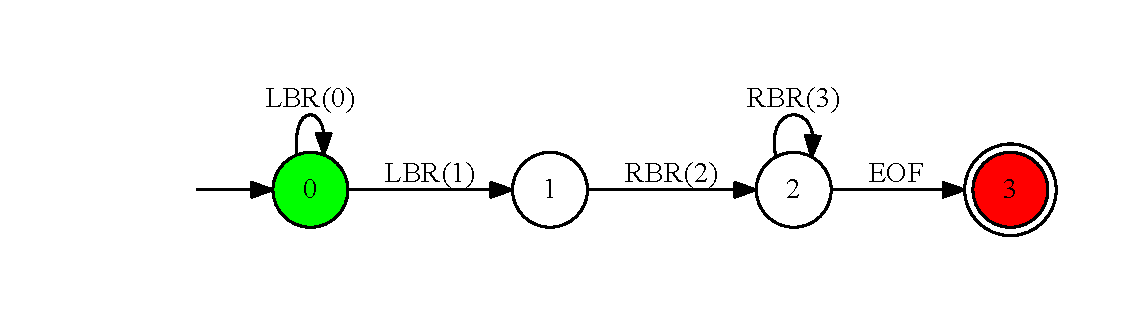
\includegraphics[width=0.38\textwidth]{part_03_GraphAnalysis/chapter_12_CFPQ/figures/07_GLR_Based/input_automaton.pdf}
    \caption{Входной граф-автомат для примера обобщённого RNGLR-алгоритма}
    \label{fig:CFPQ_GLR_input_automaton}
\end{figure}

\mytodo{Перевести обозначения на рисунке.}

Результирующий SPPF показан на рисунке~\ref{fig:CFPQ_GLR_result_sppf}.
Красным отмечены узлы, соответствующие нетерминалу $s$ для распознанных фрагментов входного графа.
Так как вход является графом, SPPF может содержать циклические зависимости и тем самым задавать потенциально бесконечное семейство деревьев вывода конечным образом.

\begin{figure}
    \centering
    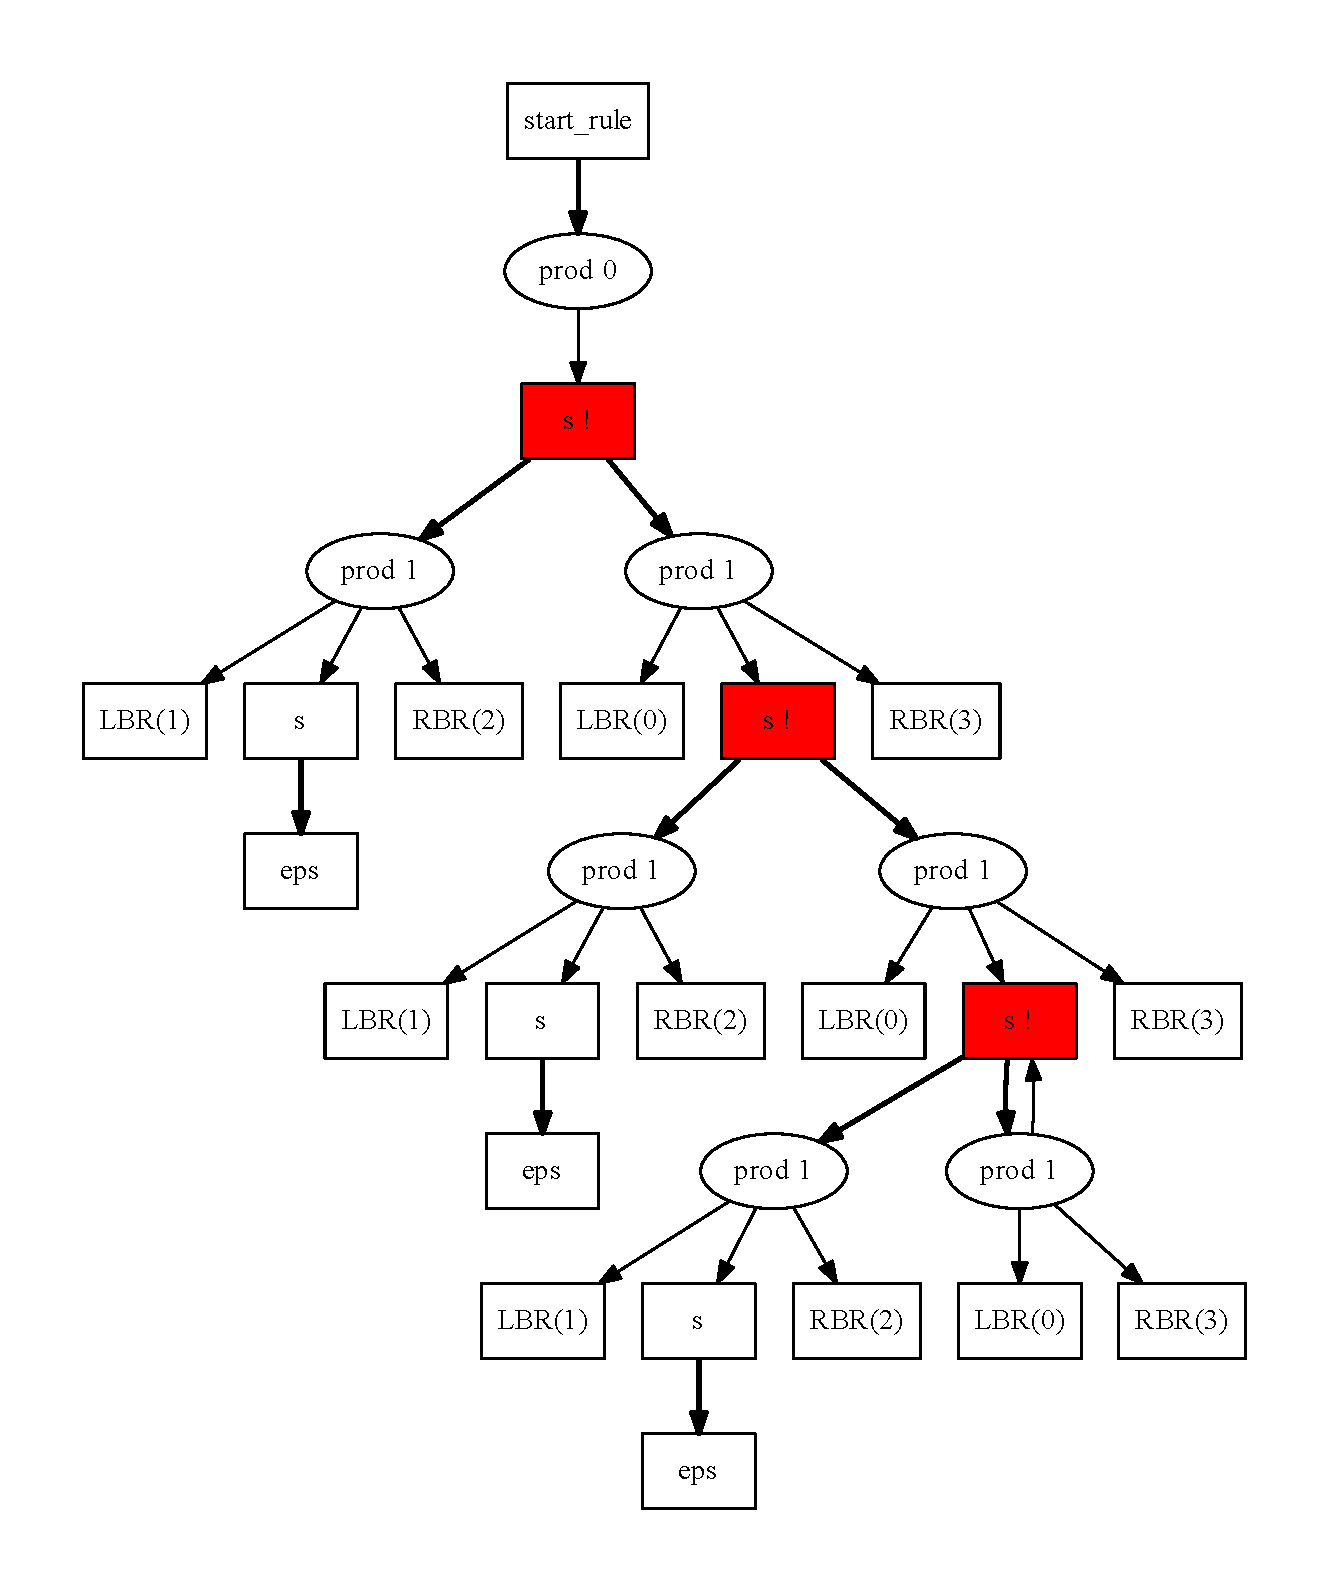
\includegraphics[width=0.72\textwidth]{part_03_GraphAnalysis/chapter_12_CFPQ/figures/07_GLR_Based/result_sppf.pdf}
    \caption{SPPF, построенный обобщённым RNGLR-алгоритмом для графа на рисунке~\ref{fig:CFPQ_GLR_input_automaton}}
    \label{fig:CFPQ_GLR_result_sppf}
\end{figure}

\mytodo{Перевести обозначения на рисунке.}

\subsection{Формальные свойства и доказательства}
\label{subsec:CFPQ_GLR_properties}
\tikzsetfigurename{CFPQ_GLR_Properties_}

\begin{theorem}[Завершимость]
    Алгоритм~\ref{algo:CFPQ_GLR_main} завершается для любого конечного входного графа и любой фиксированной КС-грамматики.
\end{theorem}

\begin{proof}
    Пусть $R$~--- множество состояний RNGLR-анализатора, а $V$~--- множество вершин входного графа.
    В каждой вершине графа может быть создано не более $|R|$ GSS-вершин, поэтому всего GSS содержит не более $|R| \cdot |V|$ вершин.
    Кратные рёбра в GSS не создаются, следовательно, число рёбер GSS конечно и ограничено квадратом числа его вершин.
    Вершины входного графа добавляются в очередь обработки только при добавлении нового ребра GSS или новой задачи, связанной с таким ребром.
    Так как число возможных GSS-рёбер конечно, основной цикл не может выполняться бесконечно.
\end{proof}

Для доказательства корректности используется понятие корректного дерева вывода для входного графа.
Такое дерево имеет стартовый нетерминал грамматики в корне, нетерминалы во внутренних узлах и терминалы в листьях, причём последовательность терминальных листьев соответствует меткам некоторого пути во входном графе.

\begin{lemma}
    Для каждого ребра GSS, связанного с узлом SPPF, терминальные листья соответствующего поддерева задают слово некоторого пути во входном графе.
\end{lemma}

\begin{proof}
    Доказательство проводится индукцией по высоте дерева вывода.
    База соответствует либо $\varepsilon$-дереву, либо дереву из одного терминала.
    В первом случае путь имеет длину ноль, во втором терминал прочитан с некоторого ребра входного графа.
    Для индукционного перехода рассмотрим дерево, корень которого помечен нетерминалом $A$, а дети соответствуют правой части некоторого правила $A \to X_1 \dots X_k$.
    По предположению индукции каждое поддерево $X_i$ соответствует некоторому пути во входном графе.
    Так как эти поддеревья получены одной свёрткой вдоль пути в GSS, конец пути для $X_i$ совпадает с началом пути для $X_{i+1}$.
    Следовательно, их конкатенация задаёт путь во входном графе для всего дерева.
\end{proof}

\begin{theorem}[Звуковость]
    Каждое дерево, восстанавливаемое из построенного SPPF, является корректным деревом вывода для некоторого пути во входном графе.
\end{theorem}

\begin{proof}
    Структура узлов SPPF гарантирует, что внутренние узлы соответствуют нетерминалам грамматики, а продукционные узлы~--- правилам грамматики.
    Остаётся проверить соответствие терминальных листьев пути во входном графе.
    Это следует из предыдущей леммы для GSS-рёбер, из которых формируется результирующий SPPF для принимающих состояний в финальных вершинах графа.
\end{proof}

\begin{theorem}[Полнота]
    Для каждого пути во входном графе, слово которого выводимо из стартового нетерминала грамматики, построенный SPPF содержит соответствующее дерево вывода.
\end{theorem}

\begin{proof}
    Доказательство повторяет доказательство полноты RNGLR для строки, за исключением одного места.
    В классическом RNGLR GSS строится послойно по позициям входной строки: к моменту обработки позиции $i$ все предыдущие уровни уже зафиксированы.
    В графе это свойство нарушается, поскольку новое ребро может появиться в уже существующей части GSS и открыть новый путь для свёртки, которая ранее уже была применена.
    Алгоритм сохраняет проходящие свёртки в вершинах GSS и при добавлении нового ребра продолжает все свёртки, которые должны пройти через это ребро.
    Поэтому ни один путь GSS, соответствующий корректному дереву вывода для пути входного графа, не теряется, а значит соответствующее дерево будет представлено в SPPF.
\end{proof}

Точная асимптотическая оценка времени работы обобщённого алгоритма зависит от способа поиска путей в GSS при свёртках, от числа повторных обработок проходящих свёрток и от размера строящегося SPPF.
В исходной работе подчёркивается, что полная оценка сложности требует отдельного анализа.
Тем не менее из доказательства завершимости следует конечная верхняя граница на число GSS-вершин и GSS-рёбер: при $|R|$ состояниях анализатора и $|V|$ вершинах входного графа число GSS-вершин не превосходит $|R| \cdot |V|$, а число GSS-рёбер~--- $O((|R| \cdot |V|)^2)$.
Если требуется только факт существования пути, можно остановиться после обнаружения принимающей GSS-вершины в финальной вершине графа; если требуется представление всех путей, необходимо построить и сохранить соответствующий SPPF.
